\documentclass[twoside,colorback,accentcolor=tud4c,11pt]{tudreport}
\usepackage{ngerman}
\usepackage[utf8]{inputenc} 
\usepackage[T1]{fontenc}
\usepackage{siunitx}
\usepackage{hyperref}
\usepackage{units}
\usepackage{upgreek}
\usepackage{amsmath}
\usepackage{graphicx}
\usepackage{float}
\usepackage[figure]{hypcap}
\usepackage{isotope}
\usepackage{subfig}

\title{Versuch 4.3: Kühlen und Fangen von Rubidium-Atomen in einer MOT}
\subtitle{	\begin{tabular}{p{8cm}ll}
Dominik Pfeiffer   &   Jonas Fischer \\ Matrikelnummer: 2913632  &   Matrikelnummer: mnr       \\ email: \textaccent{ dominik@diepfeiffers.de} & email: \textaccent{email}  
			\end{tabular} }
\subsubtitle{ \\Versuchsbetreuung : Dominik Schäffner \\ Datum der Durchführung: 26.06.2017 \\ Abgabetermin:17.07.2017    }
\institution{Praktikum für Fortgeschrittene}
\sponsor{Hiermit erklären wir, dass wir die vorliegende Arbeit bzw. Leistung eigenständig, ohne fremde Hilfe und nur unter Verwendung der angegebenen Hilfsmittel angefertigt haben. Alle übernommenen Textstellen aus der Literatur beziehungsweise dem Internet sind als solche kenntlich gemacht. Diese Arbeit hat in gleicher oder ähnlicher Form noch keiner Prüfungsbehörde vorgelegen. \\\\ 
\begin{tabular}{lp{2em}lp{2em}l}
 \hspace{4cm}   && \hspace{4cm}  && \hspace{4cm}
 \\\cline{1-1}\cline{3-3}\cline{5-5}
 Ort, Datum     && Dominik Pfeiffer && Jonas Fischer
\end{tabular}  }


\dedication{}
\lowertitleback{}
\listfiles
    
\begin{document}

\maketitle 

\tableofcontents


\chapter{Einleitung und Ziel des Versuchs}
Ziel dieses Versuches ist es schrittweise eine magnetooptische Falle (MOT) aufzubauen, $\isotope[85]{Rb}$-Atome in dieser zu fangen und die Temperatur in verschiedenen Phasen der MOT zu bestimmen. Hierfür wird zunächst das zum Kühlen verwendete Lasersystem stabilisiert, dann die Ladephase der MOT überprüft und schließlich die zur Temperaturbestimmung notwendigen Messungen durchgeführt.

\chapter{Physikalische Grundlagen}
Zunächst sollen der Aufbau und dessen wichtigste Komponenten, sowie die Theorie hinter der Laserkühlung bis in den unteren Mikrokelvinbereich und das räumliche Fangen in der Falle näher betrachtet werden.
\section{Aufbau und wichtige Komponenten}
Zunächst betrachten wir den Versuchsaufbau, der sich im wesentlichen in drei Bereiche aufteilen lässt. Zunächst ist für die Datenaufnahme ein PC mit angeschlossenem digitalen Oszilloskop und einem zusätzlichen Monitor für die Live-Darstellung der Bilder der CCD-Kamera vorhanden. Des Weiteren ist die komplette Steuerungstechnik mit allen wichtigen Komponenten zur Steuerung der Laser, Magnetspulen und Kameras in einem Elektronik-Rack untergebracht. Darunter auch die drei analogen Oszilloskope, die zur Laserstabilisierung benötigt werden. Den dritten Bereich bildet der optische Aufbau, welcher komplett auf einem optischen, möglichst schwingungsarm gelagerten Tisch montiert ist, siehe Abbildung \ref{aufb}:
\begin{figure}[H]
\centering
   	\begin{minipage}[b]{0.85\textwidth}
   	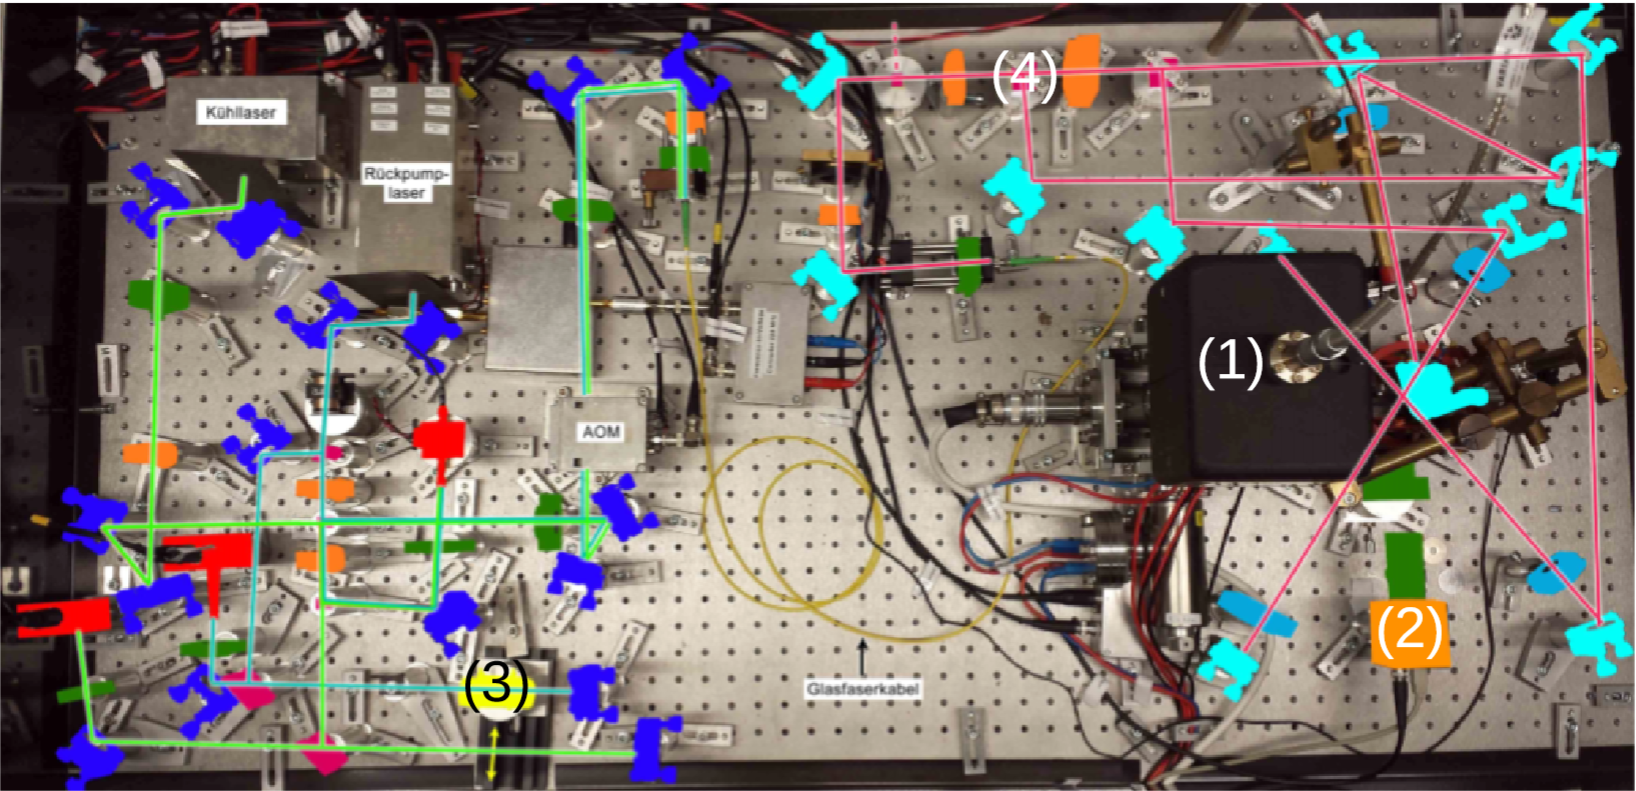
\includegraphics[width=\textwidth]{graphics/aufbau2.png}\
   	\end{minipage}
\caption{Bild von oben auf den optischen Tisch mit dem Aufbau, sowie den eingezeichneten Strahlengängen \cite{anl}}\label{aufb}	
\end{figure}
Folgend sollen die wichtigsten Komponenten des optischen Aufbaus und ihre Funktion kurz erläutert werden. Dabei wird Bezug auf die obige Abbildung genommen, in der einige Komponenten bereits eine Beschriftung tragen, andere sind farblich und/oder mit einer Nummer gekennzeichnet.
\subsection{Akusto-Optischer-Modulator (AOM)}
Der AOM ist im Aufbau in der Mitte zu sehen und trägt ebendiese Aufschrift. Dieses Bauteil besteht aus einem Kristall, einem Ultraschall-Piezoelement und einem Dämpfer. Durch das Piezoelement wird eine Ultraschallwelle in den Kristall der Frequenz $f_{AOM}=96\,\si{MHz}$ eingestrahlt, welche am anderen Ende des Kristalls vom Dämpfer absorbiert wird, wodurch das Entstehen stehender Wellen verhindert wird. Wird der Laser in den AOM eingestrahlt, sieht er aufgrund der durch die Schallwelle im Kristall verursachte Dichte- und damit Brechungsindex-Schwankung ein sich bewegendes optisches Gitter. In der ersten Beugungsordnung dieses Gitters wird die um die Frequenz des AOMs blauverschobene Laserstrahlung ausgestrahlt. Im Versuch dient der AOM hauptsächlich als Schalter, um den Laserstrahl gezielt an-/ausschalten zu können.
Die Kamera (2) wird dazu verwendet, um ein stetiges Live-Bild der MOT auf einem extra Monitor darstellen zu können. Dies ist notwendig um im Laufe des Versuches während der Messungen die korrekte Funktion der MOT überprüfen zu können und Notfalls die Messung zu stoppen um eventuelle Fehler zu korrigieren.
\subsection{PID-Regler}
Im Versuch kommen für die Stabilisierung der beiden Laser s.g. PID-Regler zum Einsatz. Diese Verarbeiten ein elektronisches Eingangssignal auf drei Weisen und geben eine Korrekturgröße aus. Die Regler Verarbeiten die Signale dabei wie folgt:
\begin{itemize}
\item[P]: Der $\textbf{P}$roportionale Teil reagiert sehr schnell und vergleicht den Istwert $x_i$ mit dem Sollwert $x_s$. Er gibt eine Regelgröße $y$ aus, welche proportional zur Abweichung von $x_i$ gegenüber $x_s$ ist. Der Nachteil dieser Methode ist es, dass nicht alle Abweichungen beseitigt werden können.
\item[I]: Der $\textbf{I}$ntegrierende Teil gibt eine Regelgröße $y$ aus, welche sich aus dem zeitlichen Integral über die Abweichung von $x_i$ gegenüber $x_s$ ergibt. Er reagiert eher langsam, beseitigt jedoch auch die kleinen Abweichungen, die der P-teil nicht beseitigen kann.
\item[D]: Der $\textbf{D}$ifferentierende Teil gibt eine Regelgröße aus, die über die Ableitung der Abweichung von $x_i$ gegenüber $x_s$ nach der Zeit ermittelt wird. Da er dabei die Geschwindigkeit der Änderung der Abweichung verwendet reagiert er sehr schnell, erkennt jedoch zeitlich konstante Abweichungen nicht.
\end{itemize}
Die Kombination der drei Einzelmodule macht den PID-Regler zu einem schnellen und effizienten Regler, weshalb er bei diesem Versuch für die Laserstabilisierung eingesetzt wird.
\subsection{Faraday-Isolator}
$\cdots$
\section{Theorie zur Laserstabilisierung}
Um in einer MOT Atome Fangen und Kühlen zu können, benötigt man verschiedene Lasersysteme. In diesem Versuch kommen zwei Halbleiter-Dioden-Laser zum Einsatz. Einer ist dafür verantwortlich, die Atome kühlen (Kühllaser), der andere sorgt dafür, das die Atome sich einem zum Kühlen geeigneten Atomaren Zustand befinden (Rückpumplaser).\\
Beide Laser sind in einem in einem Aufbau mit einem externen Resonator verbaut, was eine schnelle und präzise Korrektur der Wellenlänge möglich macht. Diese schnelle Korrektur ist von Nöten, da die beiden Laser so stabil wie möglich auf einem bestimmten Atomaren Übergang laufen sollen um die MOT stabil zu halten, effektiv zu Kühlen und Rückzupumpen. Der Rückpumplaser ist dabei in der s.g. Littman-Anordnung verbaut. Bei dieser besteht der Resonator aus der Rückseite der Diode und einem Externen Auskopplungsspiegel, welcher über einen Piezo-Motor in verstellt werden kann. Über diesen kann die Resonatorlänge und damit die Wellenlänge des Lasers eingestellt werden. Der Kühllaser ist in der Littrow-Anordnung verbaut, bei der ein Reflexionsgitter als ein Teil des Resonators fungiert. Die (-1)-Beugungsordnung des Gitters wird dabei in die Diode zurückreflekiert un die (0)-Ordnung ausgekoppelt. Hierüber findet die Wellenlängenselektion statt. Auch das Gitter wird über einen Piezo-Motor in seiner Orientierung gegenüber der Diode verstellt um so den Laser stabil auf der gewünschten Wellenlänge zu halten.\\
Um die Laser nun stabil auf einer Wellenlänge und damit stabil auf einem Atomaren Übergang des $\isotope[85]{Rb}$ zu halten werden zwei verschiedene Methoden der Stabilisierung angewendet. Die Signale der beiden Methoden werden dabei über zwei PID-Regler verarbeitet, der jeweils für den Diodenstrom und die externen Resonatoren eine Regelgöße ausgibt, um Korrekturen der Wellenlänge vorzunehmen.
\subsection{Dopplerfreie Sättigungsspektroskopie}
Die erste zum Stabilisieren des Lasersystems, genauer des Rückpumplasers, verwendete Methode ist die Dopplerfreie Sättigungsspektroskopie. Um diese näher zu erläutern, betrachten wir zunächst das Übergangs-Schema von $\isotope[85]{Rb}$ mit Fein-/ und Hyperfein-Struktur Aufspaltung der Niveaus:
\begin{figure}[H]
\centering
   	\begin{minipage}[b]{0.85\textwidth}
   	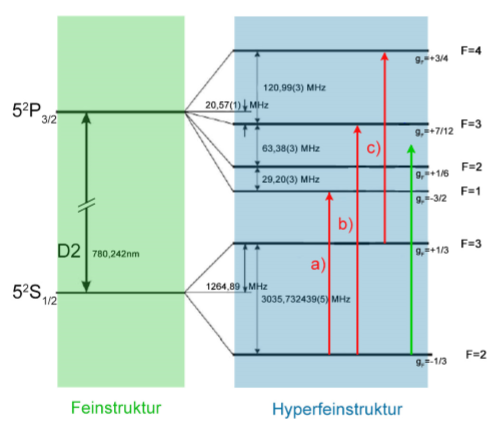
\includegraphics[width=\textwidth]{graphics/Rb_85.png}\
   	\end{minipage}
\caption{Termschema von $\isotope[85]{Rb}$ mit Fein-/ und Hyperfein-Struktur Aufspaltung sowie den verwendendeten Übergängen \cite{anl}}\label{rb85}	
\end{figure}
Der Rückpumplaser soll auf den Übergang a) in obiger Abbildung stabilisiert werden, durch die Blauverschiebung am AOM wird jedoch tatsächlich der Übergang b) zum Rückpumpen verwendet. Für die Spektroskopie wird ein Teil des Laserstrahls ausgekoppelt und durch eine Rubidiumdampfzelle hin- und zurück geleitet. Der Rücklaufende Strahl wird auf eine Photodiode geleitet, deren Signal dann elektronisch abgeleitet und über einen PID weiterverarbeitet wird. Trifft der Laser beim Durchstimmen nun genau die Frequenz eines Atomaren Übergangs, so kann dieser nur von Rubidiumatomen absorbiert werden deren Geschwindigkeit parallel zum Laserstrahl gleich Null ist, da sonst der Dopplereffekt eine Frequenzverschiebung des Laserlichts bewirkt. Aufgrund der Lebensdauer der auf dem hinweg des Laserstrahls angeregten Atome, kann auf dem Rückweg kein Laserlicht mehr absorbiert werden und es kommt zu einem Maximum der Intensität auf der Photodiode. Diese Einbrüche im Absorptionsspektrum nennt man auch Lamp-Dips.\\
Ist die Frequenz des Lasers nicht auf einem Atomaren Übergang, so können nur Rubidiumatome das Licht absorbieren, deren Geschwindigkeit parallel zum Laserstrahl genau so ist, dass durch den Dopplereffekt das Laserlicht einen Atomaren Übergang trifft. Da auf dem Hin- und Rückweg jedoch verschiedene Atome angeregt werden, kommt es zu einer höheren Absorption des Lichts, was zu einem Minimum der Intensität auf der Photodiode führt.\\
Zu einer s.g. Crossover-Resonanz (COF) und kann es kommen, wenn der Laser genau in der Mitte zweier Atomarer Übergänge eingestellt ist. Dann sind nur dieselben Atome in der Lage auf dem Rückweg das Laserlicht zu absorbieren, die bereits auf dem Hinweg angeregt wurden. Da jedoch der angeregte Zustand eine nicht verschwindende Lebensdauer hat, sinkt die Absorption auf dem Rückweg und es kommt erneut zu einem Maximum der Intensität auf der Photodiode.\\
Der Laser soll auf den $F=2\rightarrow F'=1$ Übergang stabilisiert werden. Hierfür wird der Rückpumplaser durch eine Dreiecksspannung am Piezomotor des externen Resonators in seiner Frequenz durchgestimmt und das Signal der Photodiode zunächst elektronisch abgeleitet. Ein Maximum der Intensität auf der Photodiode hat dadurch einen Nulldurchgang, auf den Der PID-Regler stabilisieren kann. 
\subsection{Offsetlock}
Der eigentliche Kühllaser wird mittels Offsetlock gegenüber dem Rückpumplaser stabilisiert und dabei dessen Stabilisierung auf einen Atomaren Übergang genutzt. Beim Offsetlock werden die beiden Laserstrahlen überlagert auf einer Photodiode abgebildet, wodurch sich ein Schwebungssignal ergibt. Dieses wird elektronisch in eine Gleichspannung umgewandelt (und vorher mit $\frac{1}{16}$ multipliziert) und auf einer Anzeige dargestellt. Im Versuch wurde für die MOT ein Offset von $f_{Offset}=2920\,\si{MHz}$ eingestellt.
\section{Theorie zur MOT}\label{theorie} 	
\chapter{Versuchsdurchführung und Auswertung}
In den Folgenden Kapitel wird sowohl die Durchführung, welche sich nach der Anleitung \cite{anl} richtet, als auch die Auswertung dargestellt. Zunächst wurde die Stabilisierung des Lasersystems durchgeführt und die Ladephase der MOT überprüft. Danach wurden zwei Messreihen an Bildern aufgenommen um die Temperatur der MOT und der optischen Melasse zu ermitteln.
\section{Stabilisierung des Lasersystems}
Zunächst müssen die Laser so stabilisiert werden, dass die MOT effizient arbeitet. Dabei verwenden wir die bereits erklärten Methoden der dopplerfreien Sättigungsspektroskopie und den Offsetlock. Für die Spektroskopie des Rückpumplasers wird eine Rubidiumdampfzelle in den Strahlengang gebracht und am PID-Regler die Dreieckspannung für den Piezomotor des externen Resonators angestellt. Das Spektroskopiesignal wurde sowohl auf einem analogen als auch auf einem digitalen, mit dem PC verbundenen Oszilloskop dargestellt und Betrachtet. in Abbildung \ref{spek1} ist ein enger Ausschnitt, in Abbildung \ref{spek2} ein etwas weiterer Ausschnitt des Signals zu sehen. Die große Anzahl der Messpunkte zu einer Piezospannung kommt dadurch zustande, dass die Dreiecksspannung in einer hohen Geschwindigkeit durchgefahren wird und sich dadurch mehrerer Messreihen überlagern. Deshalb wurde zusätzlich der Durchschnitt berechnet und dargestellt. Gut zu erkennen ist der COF-Peak und links daneben der eigentlichen Peak des atomaren $F=2\rightarrow F'=1$ Übergangs.
\begin{figure}[H]
  \centering
  \subfloat[Enger Ausschnitt des Spektroskopiesignals - Datenpunkte und Durchschnitt]{\label{spek1}
    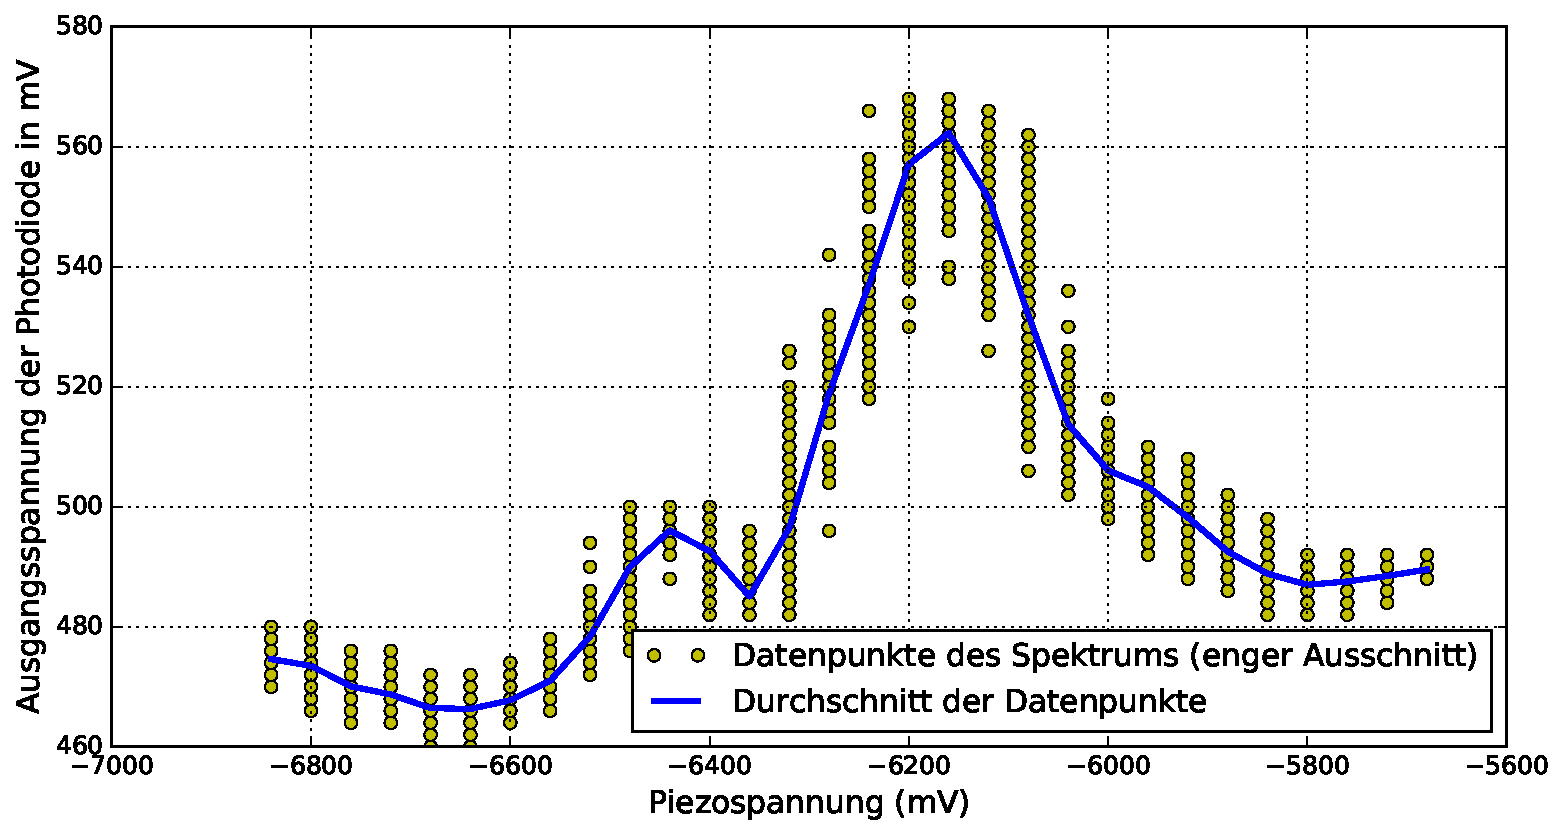
\includegraphics[width=0.48\textwidth]
    {graphics/spek1.pdf}}\quad
  \subfloat[Weiter Ausschnitt des Spektroskopiesignals - Datenpunkte und Durchschnitt]{\label{spek2}
    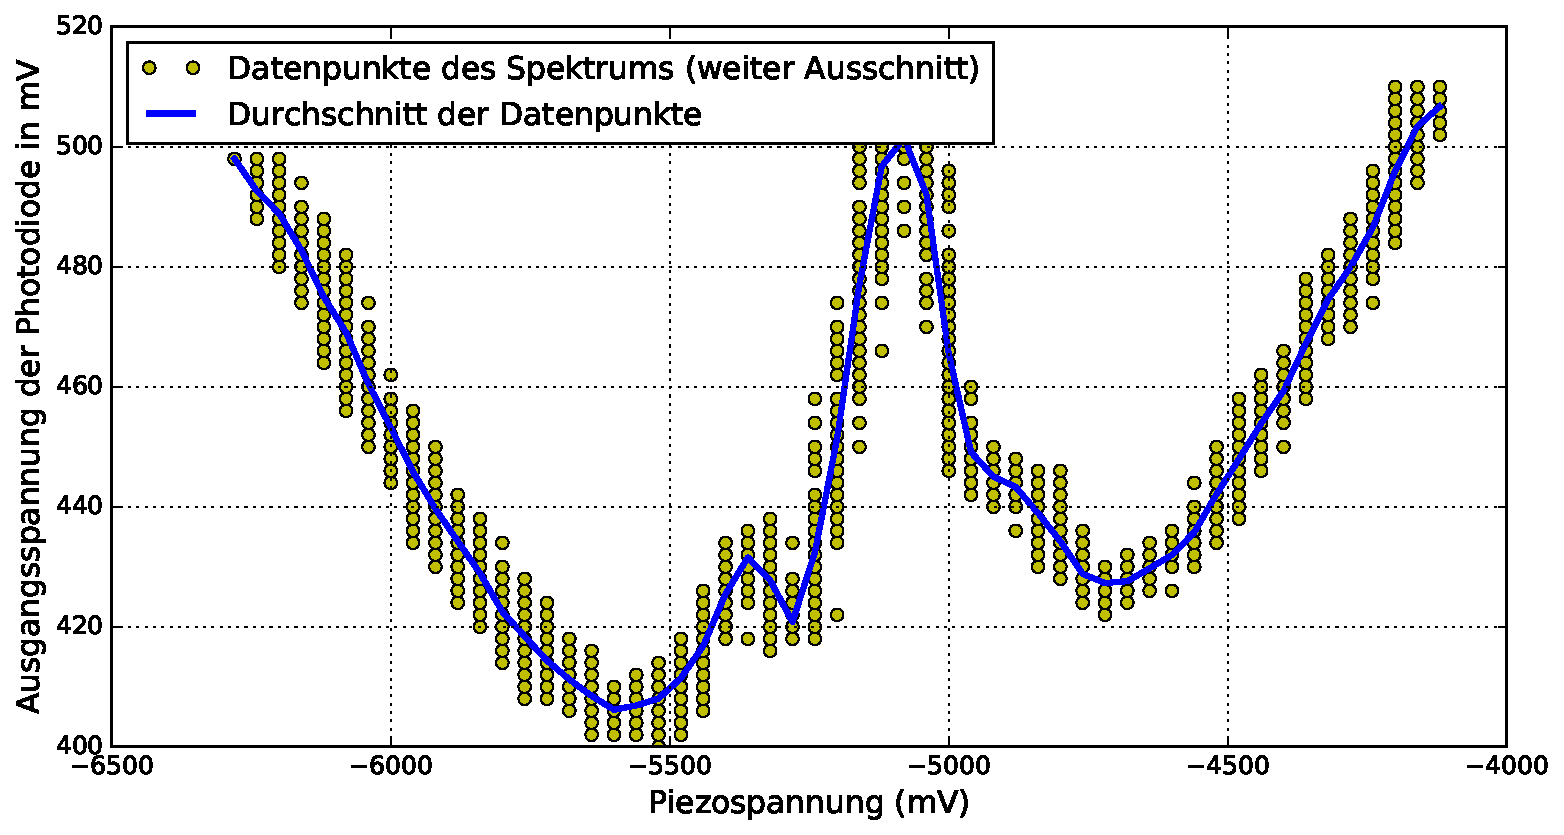
\includegraphics[width=0.48\textwidth]
    {graphics/spek2.pdf}}\quad
  \caption{Bei der dopplerfreien Sättigungsspektroskopie aufgenommene Spektren - Datenpunkte und Durchschnitt aufgetragen über der Spannung am Piezomotor}
  \label{spektren}
\end{figure}
Um den Rückpumplaser zu stabilisieren wurde das Dispersionssignal, was dem von einem Lock-In-Verstärker abgeleiteten Spektroskopiesignal entspricht, ebenfalls zunächst auf einem analogen Oszilloskop betrachtet und dann über ein digitales Oszilloskop an den PC übermittelt. Die zu Betrachtende Flanke mit dem Nulldurchgang ist in Abbildung \ref{flanke} zu sehen. Diese Abbildung stellt nur einen Ausschnitt aus dem gesamten Dispersionsignal dar.
\begin{figure}[H]
  \centering
  \subfloat[Flanke des Dispersionssignals - Datenpunkte und Durchschnitt]{\label{flanke}
    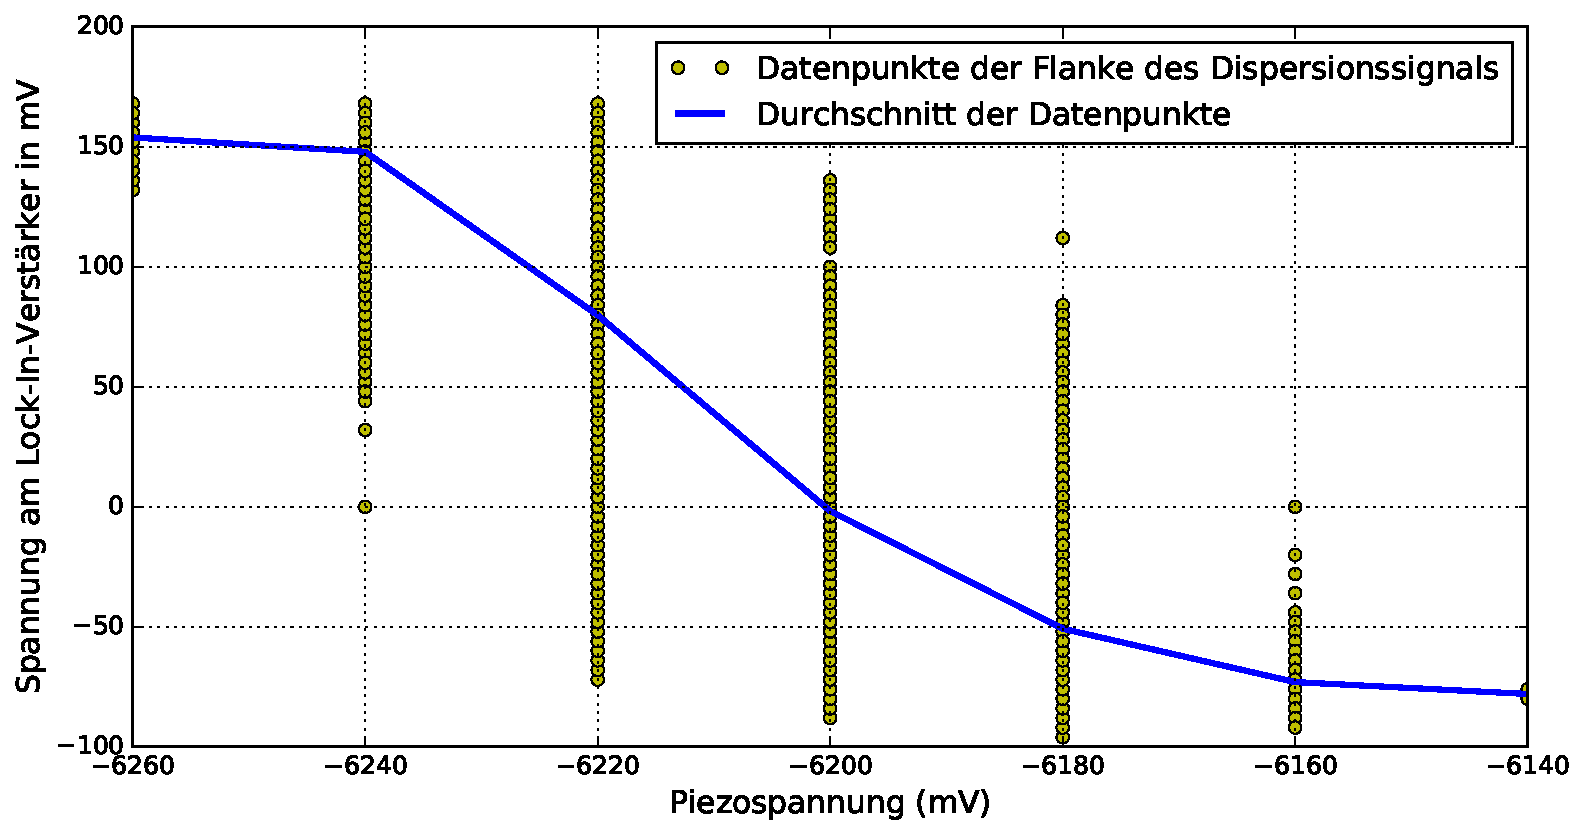
\includegraphics[width=0.48\textwidth]
    {graphics/flanke.pdf}}\quad
  \subfloat[Offsetsignal - Datenpunkte und Durchschnitt]{\label{offset}
    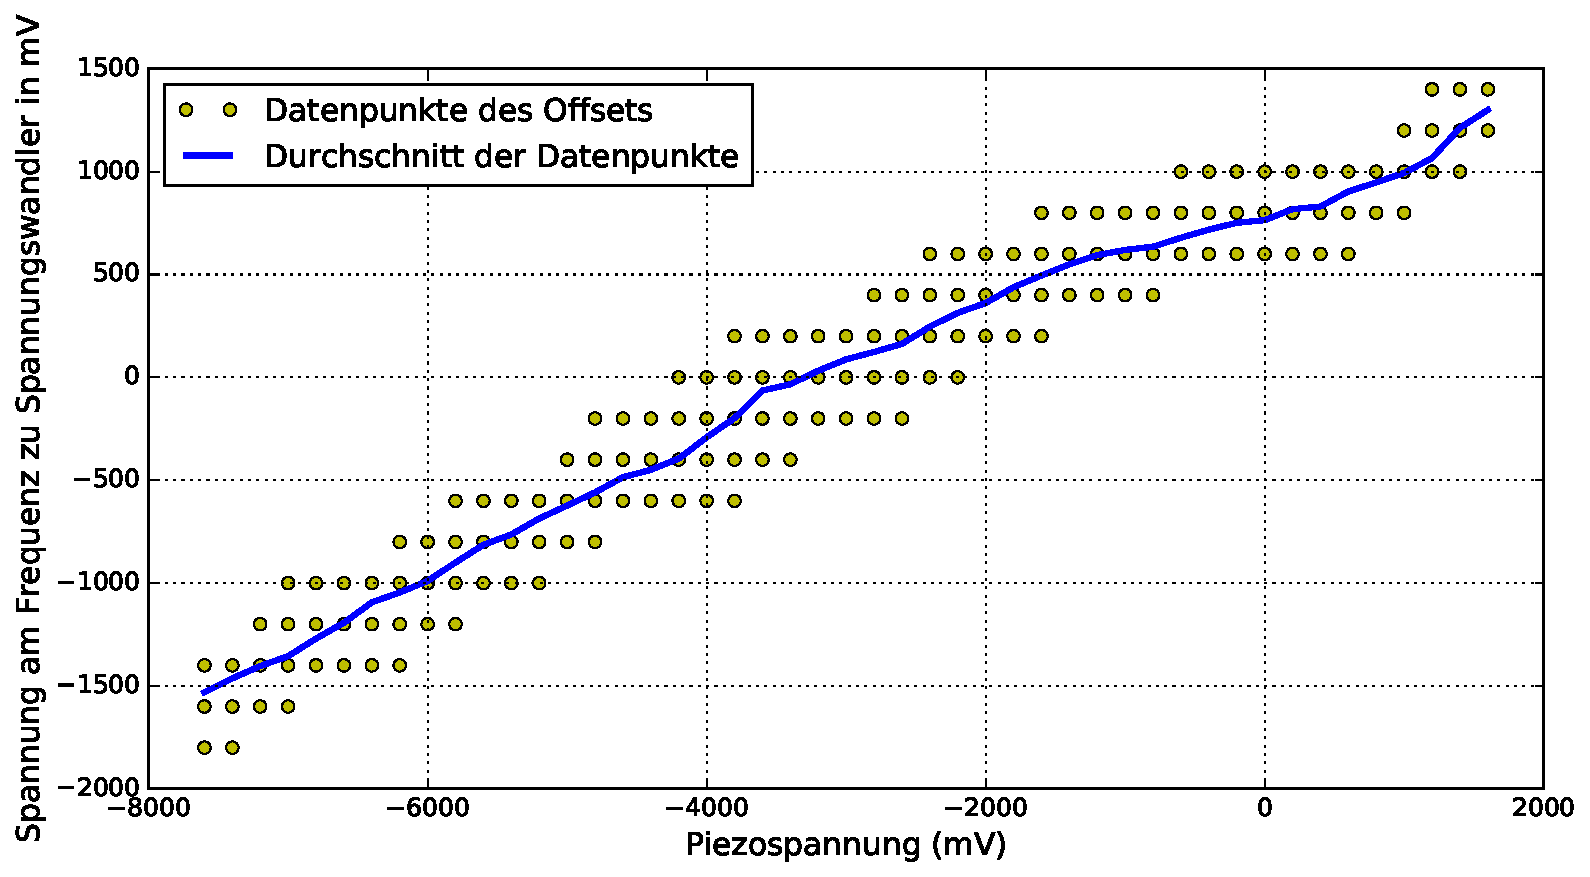
\includegraphics[width=0.48\textwidth]
    {graphics/ofset.pdf}}\quad
  \caption{Die Datenpunkte und Durchschnitte der Flanke des Dispersionssignals sowie des Offsetsignals aufgetragen über der Spannung am Piezomotor}
  \label{fldis}
\end{figure}
Nachdem der Rückpumplaser erfolgreich auf den gewünschten atomaren Übergang stabilisiert werden konnte, wurde der eigentliche Kühllaser mittels des Offsetlock stabilisiert. Das in eine Gleichspannung umgewandelte Schwebungssignal aufgetragen über die Spannung am Piezomotor des externen Resonators des Kühllasers ist in Abbildung \ref{offset} zu sehen. Da die PID-Regler immer auf einen Nullwert Regeln, wurde die Offset-Gerade so lange verschoben, bis der gewünschte Wert auf dem Nulldurchgang lag.
\section{Ladephase der MOT}
Nachdem das Lasersystem erfolgreich stabilisiert werden konnte, wurde im nächsten Schritt die Ladephase der MOT überprüft. Hierfür wurde Schrittweise die Ladezeit von $t_{Laden}=1\,\si{s}$ auf $t_{Laden}=20\,\si{s}$ in $\Delta t_{Laden}=1\,\si{s}$ Schritten erhöht. Nach Ablauf der Zeit wurde automatisch ein Bild mit einer angeschlossenen USB-Kamera aufgenommen. Durch das Betrachten der so erstellten Bilder konnte abgeschätzt werden, ob alles richtig funktioniert und ab wann in der MOT eine ausreichende Menge an Atomen gefangen wurde. Wir haben uns in Absprache mit dem Betreuer für $t_{Lade}=15\,\si{s}$ entschieden. 
\begin{figure}[H]
\centering
   	\begin{minipage}[b]{0.85\textwidth}
   	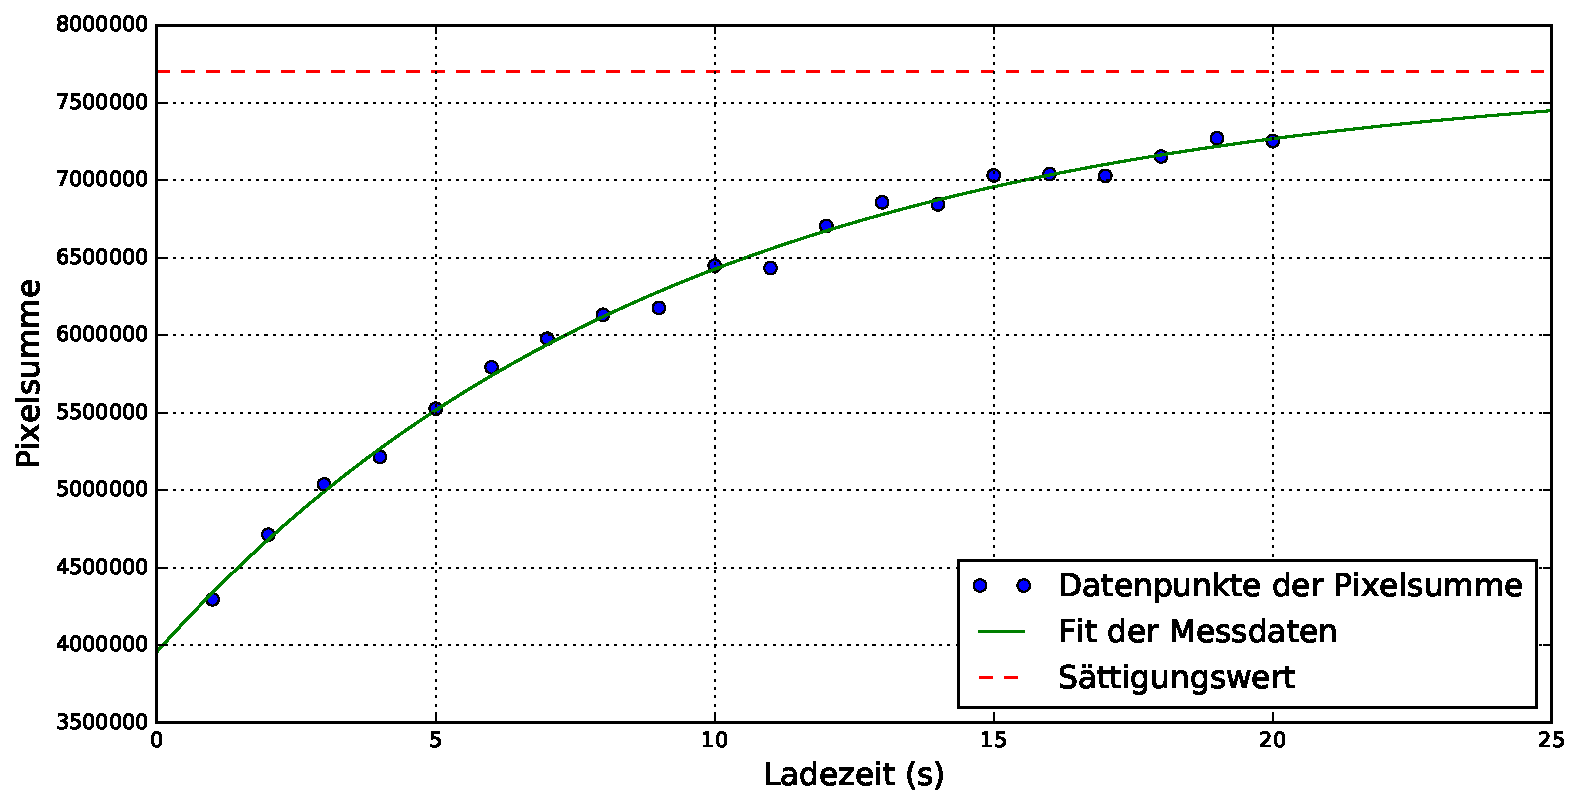
\includegraphics[width=\textwidth]{graphics/laden.pdf}\
   	\end{minipage}
\caption{Ladephase der MOT - Dargestellt sind die aufsummierten Pixelwerte der Kamera nach der jeweiligen Ladedauer mit der an die Datenpunkte angefertigten Fitfunktion und dem Sättigungswert}\label{laden}	
\end{figure}
Durch berechnen der Summe über alle Pixelwerte der einzelnen Bilder, auftragen dieser über der Ladezeit und fitten einer Funktion der Form
\begin{equation}
f(t)=A\cdot\left(1-\exp\left(-\beta\cdot t\right)\right) + B,
\end{equation}
wobei A die Amplitude, $\beta$ ein Dämpfungsfaktor und B ein zeitlich konstantes Offset (Hintergrund-Streulicht) darstellen, konnte diese Entscheidung im Nachhinein bestätigt werden. Es ergaben sich $A=3,75\cdot 10^6 \pm 1$, $\beta=0,107\pm 0 \frac{1}{s}$ und $B=3,96\cdot 10^6 \pm 1$ und damit ein Sättigungswert von $\approx7,7\cdot 10^6$. Nach $t_{Lade}=15\,\si{s}$ wurden 91,3\% des Sättigungswertes erreicht.
\section{Temperaturbestimmung in der MOT}
Um die Temperatur des Atomensembles in der MOT bzw. in der optischen Melsasse der MOT zu bestimmen gehen wir wie folgt vor:
\begin{itemize}
\item[1)] Zunächst werden die Pixelwerte der Bilder entlang einer Bildachse aufsummiert. Bei der Auswertung konnte dies nur entlang der vertikalen Bildachse als sinnvoll erachtet werden, da sich aufgrund des Störlichts im unteren Linken Eck der aufgenommenen Bilder entlang der horizontalen Bildachse keine Struktur des Atomensembles aus dem Störlicht filtern lies.
\item[2)] Im nächsten Schritt wird eine Gauss-Funktion über die Verteilung gelegt, deren x-Achse über die Angabe, dass ein Pixel eine Breite von $b_{Pixel}=6,7\,\si{\mu m}$ hat in Meter umgerechnet wurde. An die Pixelwertverteilungen der Bilder wurde die Funktion
\begin{equation}
f(x)=A\cdot\exp\left(-\frac{(x-x_0)^2}{2\sigma^2}\right) +B 
\end{equation}
angepasst. Dieser Schritt wurde für jedes der Einzelbilder der Messreihen durchgeführt.
\item[3)] Das Ensemble der $\isotope[85]{Rb}$-Atome kann hinsichtlich seiner Geschwindigkeit über die Maxwell-Boltzmann-Verteilung beschrieben werden. Diese ist gegeben durch:
\begin{equation}
f_{MB}(v_x)=4\pi v^2\cdot C\cdot\exp\left(-\frac{mv_x^2}{2k_BT}\right)
\end{equation}
\item[4)] Durch einen Vergleich der Exponenten und ausnutzen der Tatsache, das gilt $v_x=\frac{x-x_0}{t}$ ergibt sich
\begin{align}
\rightarrow\frac{(x-x_0)^2}{2\sigma^2}&=\frac{mv_x^2}{2k_BT}\\
\leftrightarrow\sigma^2&=\frac{k_BT}{m}\cdot t^2
\end{align}
Trägt man also nun die sich aus den Gauss-Fits ergebenden $\sigma^2$-Werte über dem Quadrat der zugehörigen Flugzeit $t_{Flug}$ auf, so erhält man im Idealfall eine Gerade, aus deren Steigung sich die Temperatur des Atomensembles über $T=\frac{m_{Gerade}\cdot m_{Atom}}{k_B}$ berechnen lässt.
\end{itemize}
\subsection{Temperatur der MOT}
Um die Temperatur des Atomensembles in der MOT ohne eine optische Melasse zu bestimmen, wurde zunächst die Ladezeit auf $t_{Lade}=15\,\si{s}$ eingestellt, die Zeit der optischen Melasse auf $t_{Melasse}=0\,\si{s}$ und dann eingestellt. Um nun die Temperatur bestimmen zu können wird nach Ende der Ladephase die Flugzeit der Atome in $0,250\,\si{\ms}$ Schritten von $0-5\,\si{ms}$ erhöht und nach Ablauf der Zeit ein Bild des Ensembles aufgenommen. Da bereits nach einer Flugzeit von nur $2,5\,\si{ms}$ auf den Bildern das Atomensemble nicht mehr erkennbar war und das Streulicht überwog, wurde die Messung beendet. Der Zyklus "`Laden-Flugphase-Bild"' wurde für jede Flugzeit vier mal durchgeführt und die Bilder zu einem gemittelt. Nach der oben beschriebenen Methode wurden dann die $(t_{Flug}^2,\sigma^2)$ Wertepaare aufgetragen und eine Ausgleichsgerade angepasst. in Abbildung \ref{tmot} Sind sowohl die Wertepaare, als auch die Ausgleichsgerade zu sehen.
\begin{figure}[H]
\centering
   	\begin{minipage}[b]{0.85\textwidth}
   	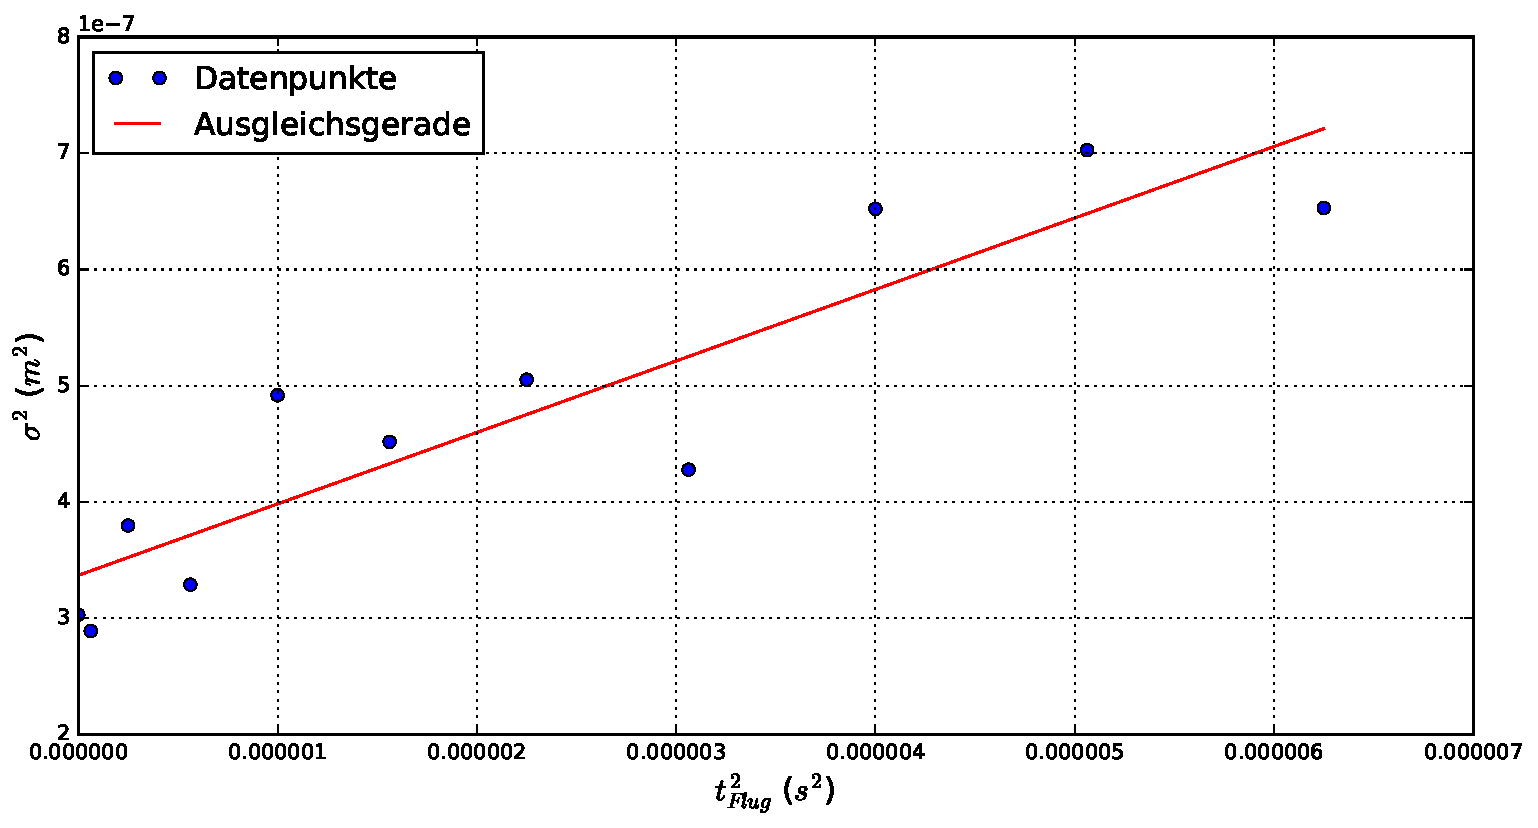
\includegraphics[width=\textwidth]{graphics/tempmot.pdf}\
   	\end{minipage}
\caption{Aufgetragen sind die $\sigma^2$-Werte über dem quadtrierten Wert der Flugzeit $t_{Flug}^2$ aus den Gaussfits an die Pixeldaten aus der Bildreihe zur Bestimmung der Temperatur in der MOT}\label{tmot}	
\end{figure}
Anhand der Steigung dieser Ausgleichsgeraden konnte die Temperatur des Atomensembles zu 
\begin{equation}
T_{MOT}=628,43\pm 15\cdot 10^{8}\,\si{\mu K}
\end{equation}
Bestimmt werden. Der sehr große Fehler dieses Wertes ist durch das Fitten der Ausgleichsgeraden an die Datenpunkte gegeben. Da diese wie in Abbildung \ref{tmot} gut zu erkennen aber eine große Streuung aufweisen, ergibt sich eine große Schar an möglichen Ausgleichsgeraden, was wiederum den Fehler der Parameter vergrößert.\\
Des Weiteren konnte das Dopplerlimit von $T_{DL}=145,47\,\si{\mu K}$ \cite{limit} nicht sehr deutlich nicht erreicht werden. Dies kann mehrerer Ursachen haben. Zunächst ist es möglich, dass eine Ungenauigkeit im Lasersystem dazu geführt hat, dass der Kühllaser nicht optimal stabilisiert war bzw. nicht auf den korrekten Wert um das Ensemble effizient zu Kühlen. Weiter fallen die großen Ladezahlen auf, welche dafür Sprechen, dass die MOT einwandfrei funktioniert hat, jedoch die Kühlzeit aufgrund des großen Atomensembles nicht ausreichte um dieses bis an das Dopplerlimit zu kühlen.\\
Im letzten Teil des Versuches soll nun eine optische Melasse untersucht werden und ebenfalls die Temperatur des Ensembles bestimmt werden.
\subsection{Temperatur in der optischen Melasse}
\begin{figure}[H]
\centering
   	\begin{minipage}[b]{0.85\textwidth}
   	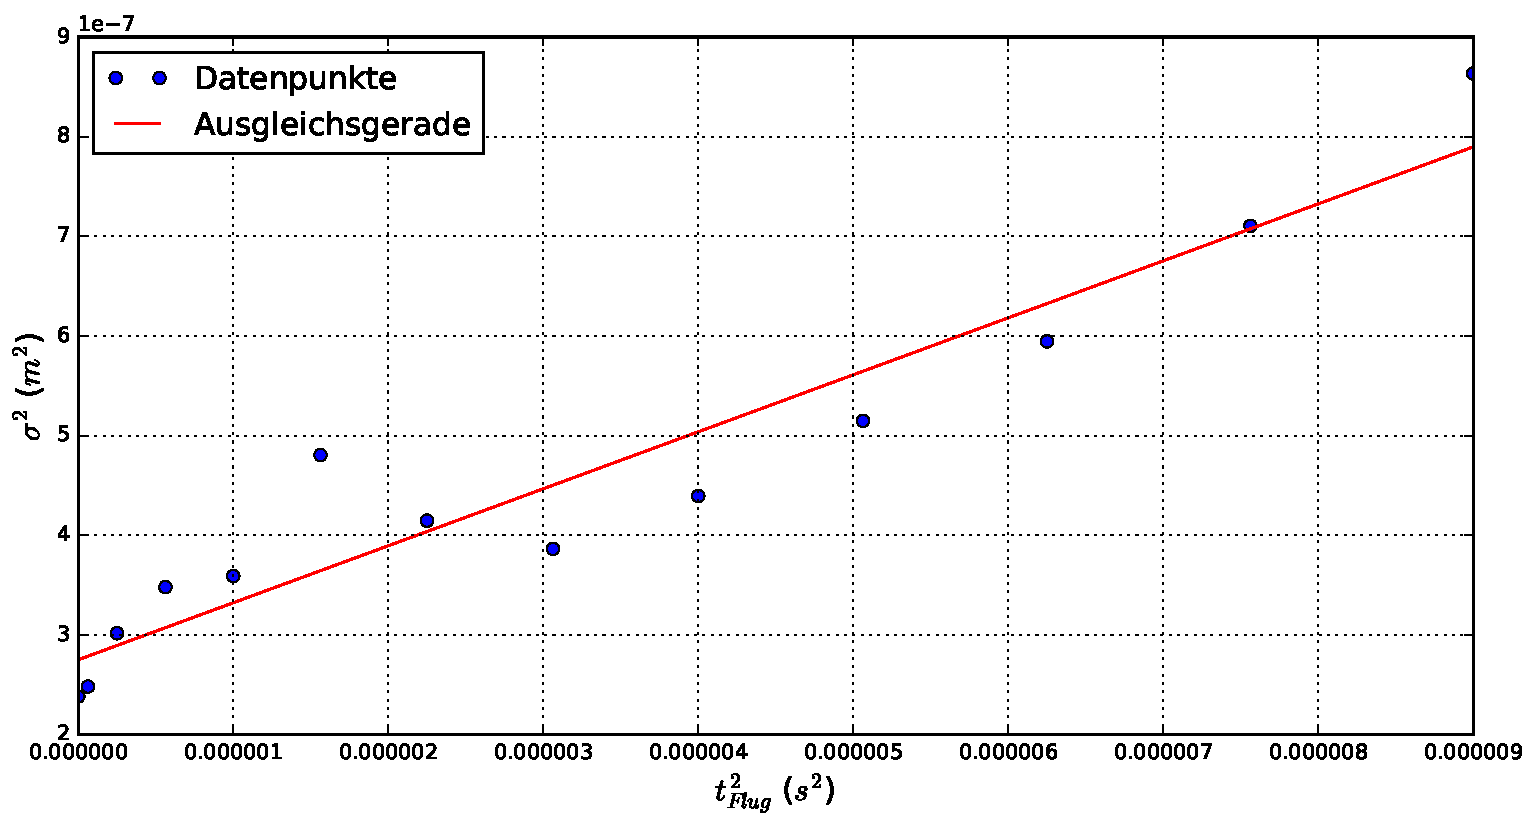
\includegraphics[width=\textwidth]{graphics/tempmel.pdf}\
   	\end{minipage}
\caption{Aufgetragen sind die $\sigma^2$-Werte über dem quadtrierten Wert der Flugzeit $t_{Flug}^2$ aus den Gaussfits an die Pixeldaten aus der Bildreihe zur Bestimmung der Temperatur in der optischen Melasse der MOT}\label{tmel}	
\end{figure}
\chapter{Diskussion}
Anhand dieses Versuches konnten einige bemerkenswerte physikalische Vorgänge eindrucksvoll Betrachtet und überprüft werden. Zunächst wurde erfolgreich das Lasersystem der MOT stabilisiert. Hierfür kamen zwei Methoden zum Einsatz, zum einen die dopplerfreie Sättigungsspektroskopie für den Rückpumplaser und auf Grundlage dessen zum anderen der Offsetlock des Kühllasers gegenüber dem Rückpumplaser.\\
Nach der Stabilisierung des Lasersystems wurde die ordnungsgemäße Funktion der MOT und der Ladeprozess überprüft. Anhand der Bilddaten und Augenmaß, sowie in Rücksprache mit dem Betreuer wurde sich für eine Ladezeit von $t_{Lade}=15\,\si{s}$ entschieden. Im Laufe der Auswertung konnte diese Entscheidung bestätigt werden, da die MOT nach $15\,\si{s}$ bereits 91,3\% des berechneten Sättigungswertes erreicht.\\
Durch die Aufnahme von Bildern nach bestimmten Flugzeiten und der Auswertung der durch die Pixeldaten der Bilder berechneten örtlichen Verteilung des Atomensembles konnte die Temperatur der MOT ohne optische Melasse zu $T_{MOT}=628,43\pm 15\cdot 10^{8}\,\si{\mu K}$ bestimmt werden. Hierbei ist der Fehler aufgrund der Ausgleichsgerade und der großen Streuung der Daten sehr groß. Des Weiteren konnte das Dopplerlimit für $\isotope[85]{Rb}$ nicht erreicht werden. Ein offensichtlicher Grund hierfür konnte nicht gefunden werden, jedoch ist ein solcher experimenteller Aufbau extrem empfindlich gegenüber äußeren Störungen, sodass eine ungenügende Justage oder eine eventuelle "`Überlladung"' der MOT mögliche Ursachen sein könnten. 





		

\renewcommand{\bibname}{Literaturverzeichnis}
\begin{thebibliography}{Bak89}
\bibitem {anl} Anleitung zum Versuch 4.3: MOT, (Stand 26.06.2017)
\bibitem {limit} http://steck.us/alkalidata/rubidium85numbers.pdf, (Zugriff: 12.07.2017)


\end{thebibliography} 	



\end{document} 
